\documentclass[
	a4paper, % Paper size, use either a4paper or letterpaper
	10pt, % Default font size, can also use 11pt or 12pt, although this is not recommended
	unnumberedsections, % Comment to enable section numbering
	twoside, % Two side traditional mode where headers and footers change between odd and even pages, comment this option to make them fixed
]{LTJournalArticle}

\addbibresource{sample.bib} % BibLaTeX bibliography file

% A shortened article title to appear in the running head, leave this command empty for no running head

% \footertext{\textit{Journal of Biological Sampling} (2024) 12:533-684} % Text to appear in the footer, leave this command empty for no footer text

\setcounter{page}{1} % The page number of the first page, set this to a higher number if the article is to be part of an issue or larger work

%----------------------------------------------------------------------------------------
%	TITLE SECTION
%----------------------------------------------------------------------------------------

\title{Probabilistic Approaches to 
\\ Energy Conservation in CDNs} % Article title, use manual lines breaks (\\) to beautify the layout

% Authors are listed in a comma-separated list with superscript numbers indicating affiliations
% \thanks{} is used for any text that should be placed in a footnote on the first page, such as the corresponding author's email, journal acceptance dates, a copyright/license notice, keywords, etc
\author{%
	Adarsh Hiremath, Artemas Radik, Andrew Palacci \\
	CS 262: Introduction to Distributed Systems \\
}


%----------------------------------------------------------------------------------------

\begin{document}

\maketitle % Output the title section

%----------------------------------------------------------------------------------------
%	ARTICLE CONTENTS
%----------------------------------------------------------------------------------------

\begin{abstract}
\end{abstract}
\section{1. Introduction}

\section{2. Existing Methods}
Notes / plans for this section: 
\begin{enumerate}
    \item 
\end{enumerate}

\section{3. The Need for a New Cache Policy}

Efficiently caching content is crucial for highly performant CDNs. Web multimedia data such as text, video, and audio can be exceptionally large, making cache policies essential for ensuring that clients receive data quickly without overburdening the surrogate servers in the CDN. In a simple 3-tier CDN model, we want to move the most popular content to the the furthest edge of the network - in this case, the 3rd tier.  

\begin{figure}[h]
	\begin{center}
		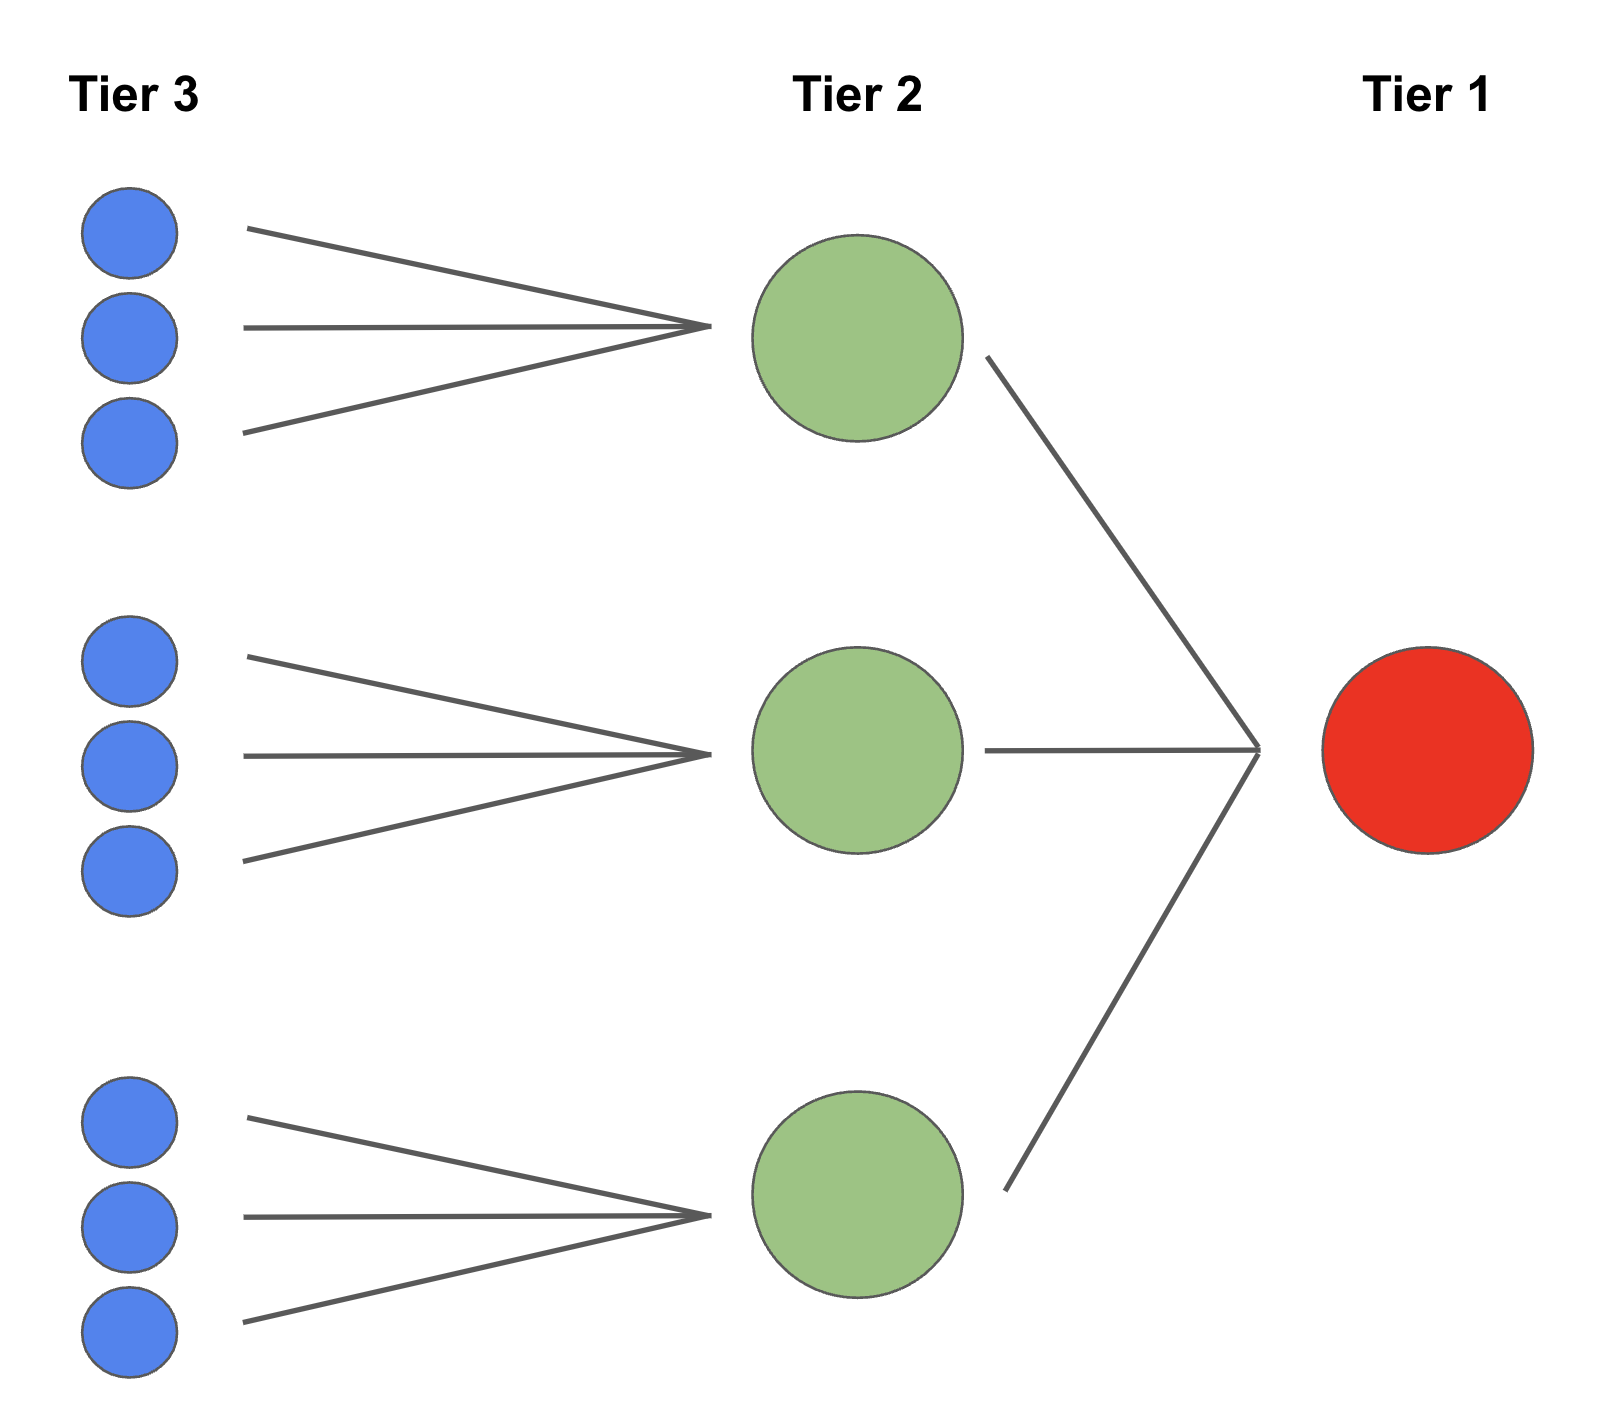
\includegraphics[width=8.1cm]{tier.png}
	\end{center}
	\caption{A diagram of a simple 3-tier CDN.}	
\end{figure}

In the above model, the primary server contains all the multimedia data to be distributed to clients. Intuitively, our goal is to minimize the amount of content near the furthest edge while minimizing cache misses to ensure that data isn't unnecessarily cached. 

\subsection{3.1 Cache-Everywhere Policies }

A naive approach to caching content on surrogate servers could be a cache-everywhere policy. In this web caching framework, a cache miss results in a chain of requests upstream to surrogate servers in order to retreive the uncached object. Once the object is found in a server's cache, the object is cached at every intermediate server between the server at the furthest edge of the network and the destination server. Cache-everywhere is observed in many older caching solutions, such as the open-source Harvest/Squid system. 

However, since every server between the edge of the network and the destination server is burdened with a new cached object in the event of a miss, this caching policy is highly inefficent. This policy is usually only employed with smaller objects under 1 kilobyte in size such as HTML pages or CSS stylesheets. Thus, cache-everywhere fails for longer forms of multimedia such as audio and video. 

\subsection{3.2 Uniformly Distributed Caches}

Another approach is to distribute cached content evenly across all surrogate servers in the network, regardless of how popular the content is. This is done by caching content uniformly. 

Although this policy ensures that all surrogate servers have a similar workload, it is not very effective because it does not consider the popularity of content. This means that highly popular content may still be located far from the furthest edge of the network, and less popular content may be replicated unnecessarily near the edge. This can lead to higher latency and longer initial response times for end clients. Thus, a uniform caching policy should be avoided in high-traffic CDNs. 

\subsection{3.3 Zipf's Law}

Cache policies can be designed to allocate caches according to different distributions. The Zipf distribution is a popular choice for determining which data to cache, as it takes the popularity of the content into account, unlike the uniform distribution.

The probability mass function (PMF) of the Zipf distribution can be mathematically expressed as:

\[
	P(X=k) = \frac{1/k^{\alpha}}{\zeta(\alpha)}
\] 

where $X$ is a random variable representing the rank of a term in a corpus, $k$ is an integer representing the rank of the term, and $\alpha$ is a parameter that controls the skewness of the distribution. $\zeta(\alpha)$ is the Riemann zeta function, defined by:

\[
	\zeta(\alpha) = \sum{k=1}^{\infty} \frac{1}{k^{\alpha}} 
\] 

Put more simply, Zipf's law states that the $k$th most popular data object will be accessed with probability $\frac{1}{k}$. A cache policy using Zipf's law would allocate cache space to surrogates based on the probability outputted by the PMF of the Zipf distribution. By taking into account the popularity of content using the Zipf distribution, Zipf's law caching is effective at minimizing cache misses and improving performance for larger multimedia data. 

\begin{figure}[h]
	\begin{center}
		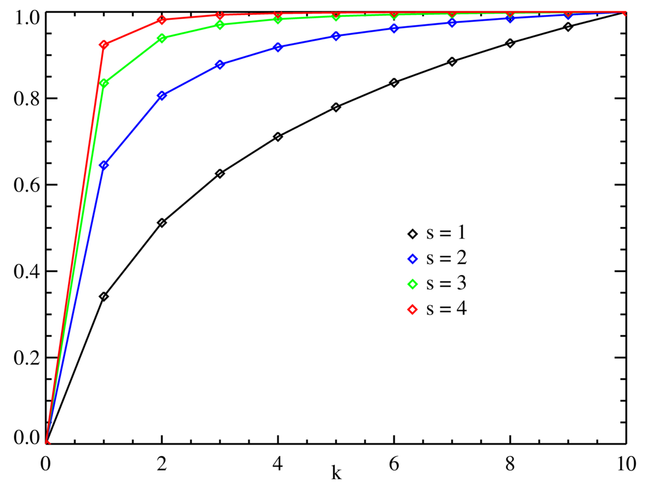
\includegraphics[width=8.1cm]{zipf.png}
	\end{center}
	\caption{A graph of the Zipf distribution CDF for $10$ elements. The horizontal axis is the $k$ parameter.}	
\end{figure}

The graph of the cumulative distribution function (CDF) of the Zipf distribution shows that the top ranked item is overweighted because the rank of each item in the Zipf distribution decreases as the rank of the item increases. This means that the probability of accessing the top-ranked item is much higher than the probability of accessing any other item. 

However, for short-form video content, such as Tik Tok and Vine, there are typically more items that have high popularity and more items that spontaneously change in popularity by going viral overnight. This means that the distribution of popularity is less skewed, and the Zipf distribution may not accurately capture the popularity of content. Therefore, using the Zipf distribution to determine cache allocation for short-form video content may not be as effective as for other types of multimedia. Other probability distributions may need to be considered to better capture the popularity of content in this specific context. Additionally, since short-form video content requires larger amounts of storage space, efficient cache allocation is even more crucial to ensure optimal performance of a CDN.

\subsection{3.4 Alternatives to Conventional Caching Policies}

In this paper, we explore two viable alternatives to the Zipf distribution for caching policy: the Pareto distribution and the bimodal distribution.

The Pareto principle, also known as the $80/20$ rule, dictates that 20\% of the content is responsible for 80\% of the views. This could be a better model for short-form video content, which is known for having viral videos that accumulate a large number of views in a short period of time. Allocating more cache space to the most popular 20\% of content using the Pareto distribution could potentially help improve the performance of a CDN for short-form video content.

The probability mass function (PMF) of the Pareto distribution can be mathematically expressed as:

\[
    P(X \geq x) = \left(\frac{x_m}{x}\right)^\alpha
\]

where $X$ is a random variable representing the size of a file, $x$ is the threshold size for caching, $x_m$ is the minimum file size for caching, and $\alpha$ is a parameter that controls the skewness of the distribution. Like the Zipf distribution, the Pareto distribution is a power law distribution, meaning that the ratio of frequencies of any two elements in the distribution is independent of the elements' actual values.  

\begin{figure}[h]
	\begin{center}
		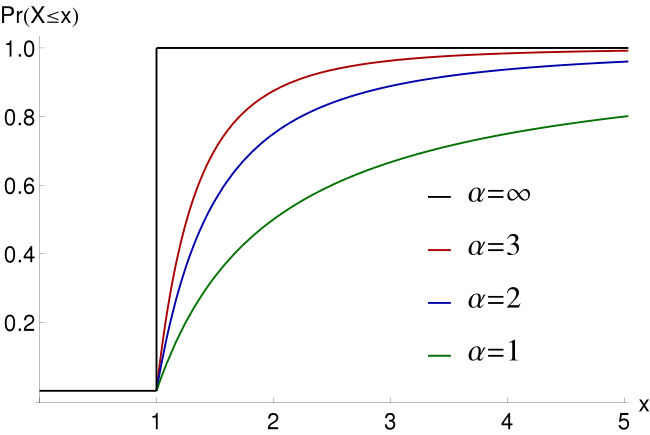
\includegraphics[width=8.1cm]{pareto.png}
	\end{center}
	\caption{A graph of the Pareto distribution CDF for various $\alpha$ with a scale parameter of $1$.}	
\end{figure}

The graph of the cumulative distribution function (CDF) of the Pareto distribution very strongly mirrors the Zipf distribution, which is to be expected because both distributions are monotonically decreasing and positively skewed. However, unlike Zipf, the Pareto distribution indicates that it takes more data objects to reach 80\% of total views. As explained in $3.3$, this addresses the primary concern with using Zipf's law to model modern multimedia. 

Another distribution that provides improvements to Zipf is the bimodal distribution. This distribution assumes that the data is comprised of two distinct groups with different levels of viewership: popular and unpopular. 

\begin{figure}[h]
	\begin{center}
		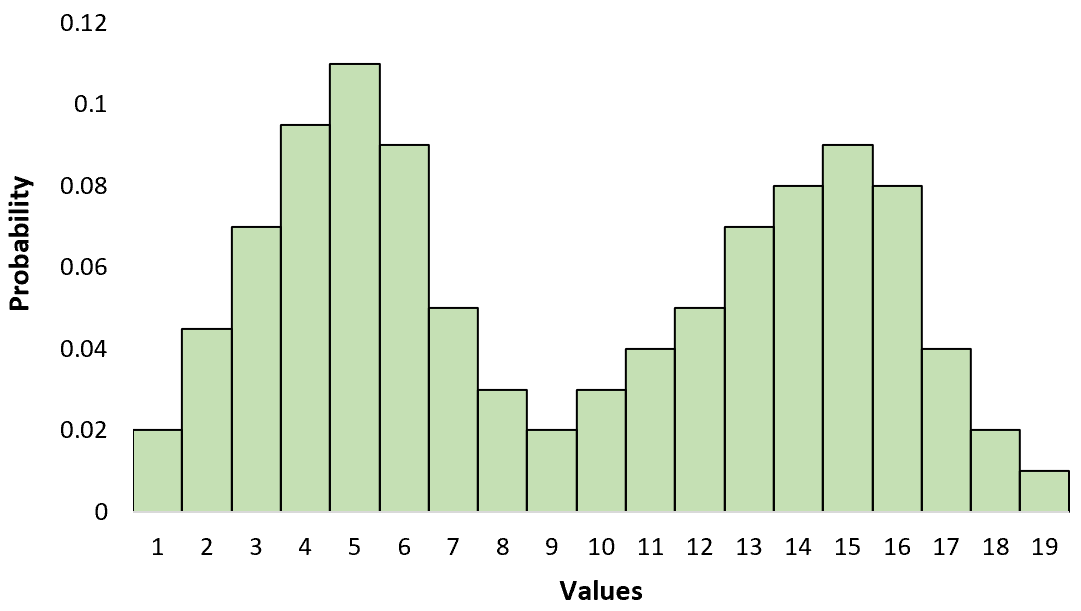
\includegraphics[width=8.1cm]{bimodal.png}
	\end{center}
	\caption{A example of data distributed bimodally with two peaks.}	
\end{figure}


As the graph of the above distribution indicates, this is a good model for today's multimedia since there is likely to be highly popular content with a large number of views and less popular content. Therefore, allocating more cache space to the highly popular content using a bimodal distribution could help improve the performance of a CDN.

% \section{x. Pareto/Bimodal Energy Consumption}

% \section{x. Samples at Scale} (potentially)

% \section{Adaptations to the current model}
% in this section, we can talk about 1. having a crossover point where adding more servers is not energy effective, 2. how we would incorporate this into our model using an additional dependency on S in the server energy 
% include a real world example analogous to the Youtube example in the current paper we are using --- use this ratio of r_m to m_m to calculate where the crossover point would be, and note that a similar strategy could be implemented by CDN users to optimize their energy consumption

% \section{x. Future Work}

% \section{x. References}


\end{document}
